\documentclass[10pt]{beamer}
\usepackage{../../shared/styles/custom}
\usepackage{../../shared/styles/conventions}
\usepackage{../../shared/notation/notation}

% Remove navigation symbols
\setbeamertemplate{navigation symbols}{}

% Add fitpic for image fitting
\newcommand{\fitpic}[1]{\begin{adjustbox}{max width=\linewidth, max totalheight=0.78\textheight}#1\end{adjustbox}}

\title{Contour Plots \& Gradients}
\date{\today}
\author{Nipun Batra and teaching staff}
\institute{IIT Gandhinagar}
\begin{document}
\maketitle

\begin{frame}{Table of Contents}
\tableofcontents
\end{frame}

\section{Understanding Contour Plots}



\begin{frame}{Introduction to Contour Plots}
\begin{definitionbox}{What is a Contour Plot?}
\textbf{Concept:} A contour plot shows curves where a function $f(x,y) = K$ for different constant values $K$
\end{definitionbox}

\onslide<2->{
    \begin{examplebox}{Function: $z = f(x,y) = x^{2} + y^{2}$}
    Circular Contours
    \end{examplebox}
}
\onslide<3->{
    \begin{center}
    \fitpic{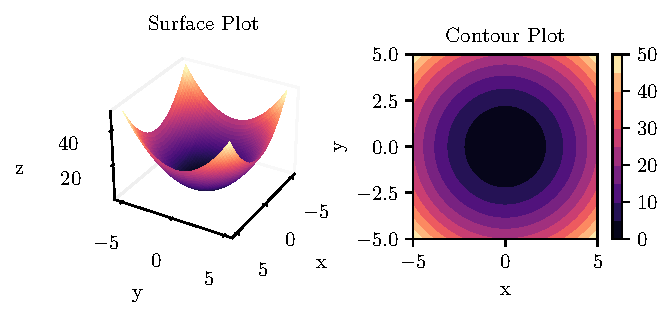
\includegraphics[width=0.7\linewidth]{../assets/mathematical-ml/figures/contour-x_squared_plus_y_squared.pdf}}
    \end{center}
}
\end{frame}
\begin{frame}{Introduction to Contour Plots}
\begin{center}
\fitpic{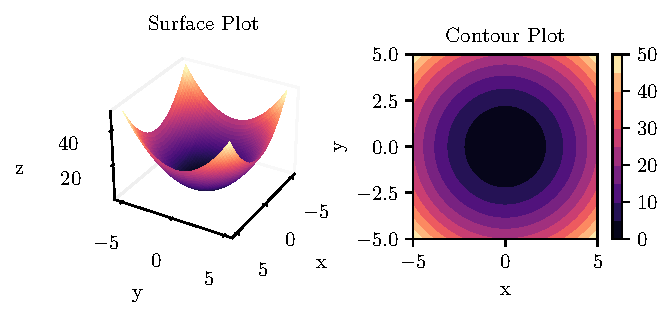
\includegraphics[width=0.8\linewidth]{../assets/mathematical-ml/figures/contour-x_squared_plus_y_squared.pdf}}
\end{center}
\onslide<2->{
    \footnotesize
    \begin{keypointsbox}
    \textbf{Key Insight:} Each contour line represents all points $(x,y)$ where $f(x,y) = K$ for a specific constant $K$
    \end{keypointsbox}
}
\end{frame}


\begin{frame}{Contour Example: Parabolic Function}
\footnotesize
\begin{examplebox}{Function: $z = f(x,y) = x^{2}$}
\textbf{Note:} This function depends only on $x$, not on $y$!
\end{examplebox}
\onslide<2->{
    \begin{center}
    \fitpic{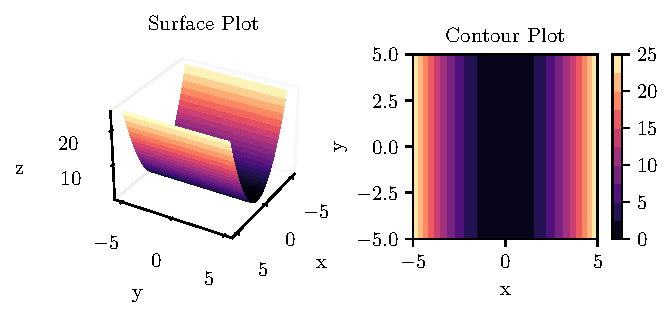
\includegraphics[width=\linewidth]{../assets/mathematical-ml/figures/contour-x_squared.pdf}}
    \end{center}
}
\end{frame}

\begin{frame}{Contour Example: Parabolic Function}
\footnotesize

\begin{center}
\fitpic{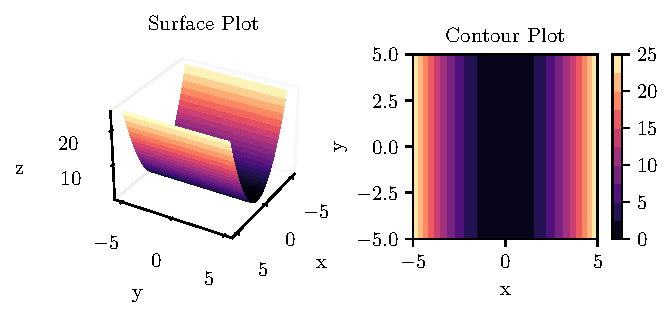
\includegraphics[width=0.7\linewidth]{../assets/mathematical-ml/figures/contour-x_squared.pdf}}
\end{center}

\begin{keypointsbox}
\textbf{Observation:} Contour lines are vertical because $f(x,y) = x^2$ is constant for all $y$ values when $x$ is fixed
\end{keypointsbox}

\onslide<2->{
    \begin{alertbox}{ML Connection}
    \textbf{This represents:} A loss function that doesn't depend on one of the parameters!
    \end{alertbox}
}
\end{frame}

\begin{frame}{Contour Example: Manhattan Distance}
\begin{examplebox}{Function: $z = f(x,y) = |x| + |y|$}
\textbf{Also known as:} Manhattan distance or L1 norm
\end{examplebox}
\onslide<2->{
    \begin{center}
    \fitpic{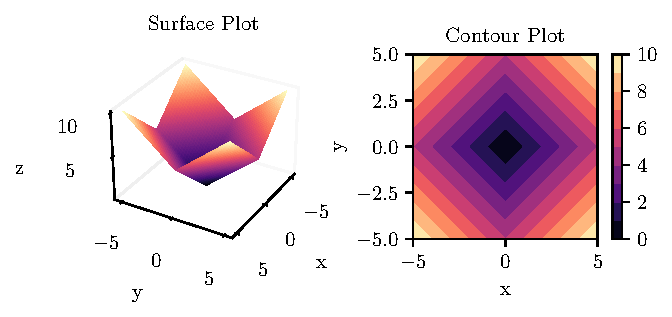
\includegraphics[width=\linewidth]{../assets/mathematical-ml/figures/contour-mod_x_plus_mod_y.pdf}}
    \end{center}
}
\end{frame}

\begin{frame}{Contour Example: Manhattan Distance}

\begin{center}
\fitpic{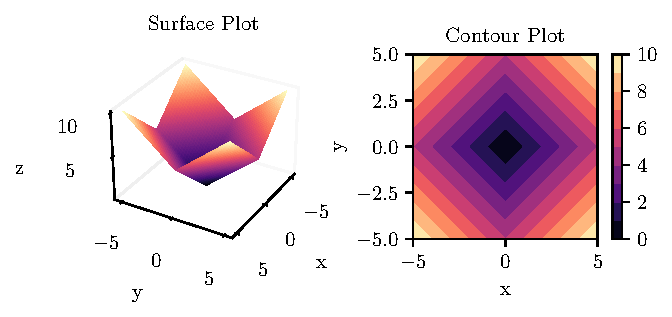
\includegraphics[width=0.7\linewidth]{../assets/mathematical-ml/figures/contour-mod_x_plus_mod_y.pdf}}
\end{center}

\begin{keypointsbox}
\textbf{Shape:} Diamond-shaped contours due to absolute value functions
\end{keypointsbox}

\begin{alertbox}{ML Connection}
\textbf{This represents:} L1 regularization in machine learning (promotes sparsity!)
\end{alertbox}
\end{frame}

\begin{frame}{Contour Example: Polynomial Function}
\begin{examplebox}{Function: $z = f(x,y) = x^2 \cdot y$}
\textbf{Type:} Mixed polynomial (quadratic in $x$, linear in $y$)
\end{examplebox}

\onslide<2->{
    \begin{center}
    \fitpic{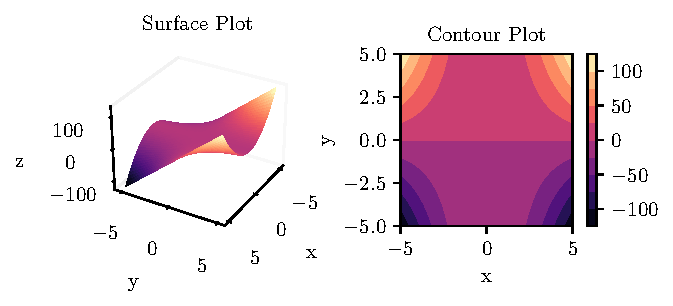
\includegraphics[width=\linewidth]{../assets/mathematical-ml/figures/contour-x_square_times_y.pdf}}
    \end{center}
}

\end{frame}

\begin{frame}{Contour Example: Polynomial Function}
\begin{keypointsbox}
\textbf{Key Features:}
\cleanitemize{
    \item Asymmetric contours
    \item Different behavior above and below $y = 0$
    \item Non-linear interaction between variables
}
\end{keypointsbox}

\onslide<4->{
\begin{alertbox}{ML Connection}
\textbf{This represents:} Complex loss surfaces with variable interactions
\end{alertbox}
}
\end{frame}

\begin{frame}{Contour Example: Hyperbolic Function}
\begin{examplebox}{Function: $z = f(x,y) = xy$}
\textbf{Type:} Bilinear function (linear in each variable separately)
\end{examplebox}

\onslide<2->{
    \begin{center}
    \fitpic{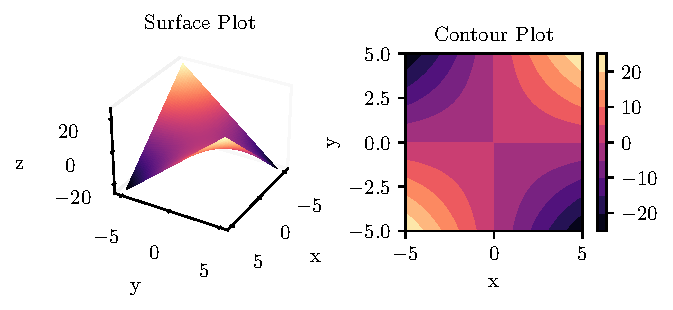
\includegraphics[width=\linewidth]{../assets/mathematical-ml/figures/contour-x_times_y.pdf}}
    \end{center}
}
\end{frame}

\begin{frame}{Contour Example: Hyperbolic Function}
\begin{center}
\fitpic{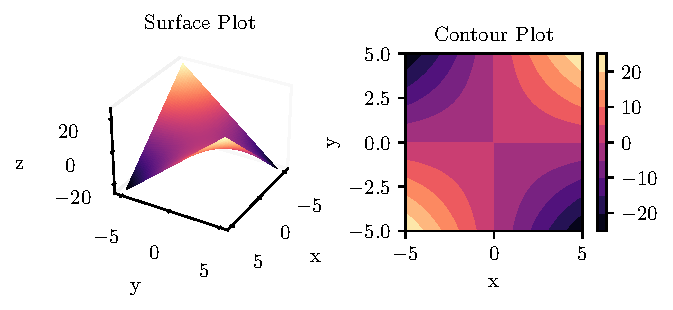
\includegraphics[width=0.7\linewidth]{../assets/mathematical-ml/figures/contour-x_times_y.pdf}}
\end{center}
\begin{keypointsbox}
\textbf{Shape:} Hyperbolic contours with saddle point at the origin
\end{keypointsbox}
\onslide<2->{
    \begin{alertbox}{ML Significance}
    \textbf{Saddle points:} Common in neural network optimization - neither minimum nor maximum!
    \end{alertbox}
}
\end{frame}


%%%%% Guntas Part %%%%%
\section{Gradients and Contour Plots}
\begin{frame}{Understanding Gradients}
\begin{definitionbox}{What is a Gradient?}
\textbf{Gradient $\grad f$:} Vector pointing in the direction of steepest increase of function $f$
\end{definitionbox}

\onslide<2->{
    \begin{keypointsbox}{Key Properties}
    \cleanitemize{
        \item \textbf{Direction:} Points toward steepest ascent
        \onslide<3->{\item \textbf{Magnitude:} Rate of steepest change}
        \onslide<4->{\item \textbf{Contour relationship:} Always perpendicular to contour lines}
    }
    \end{keypointsbox}
}
\end{frame}

\begin{frame}{Understanding Gradients}
\begin{examplebox}{Fundamental Insight}
\textbf{All points on the same contour have identical $f(x,y)$ values}\\
\onslide<2->{\textbf{Moving along a contour:} No change in function value}\\
\onslide<3->{\textbf{Moving perpendicular to contour:} Maximum change in function value}
\end{examplebox}

\onslide<4->{
    \begin{alertbox}{ML Application}
    \textbf{Gradient descent:} Move opposite to gradient direction to minimize loss!
    \end{alertbox}
}
\end{frame}

\begin{frame}{Gradients Visualized: Circular Contours}
\begin{examplebox}{Function: $z = f(x,y) = x^{2} + y^{2}$}
\onslide<2->{\textbf{Gradient:} $\grad f = \begin{bmatrix} 2x \\ 2y \end{bmatrix}$}
\end{examplebox}

\onslide<3->{
    \begin{center}
    \fitpic{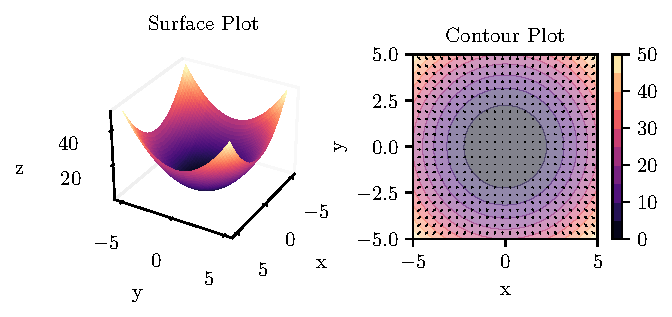
\includegraphics[width=\linewidth]{../assets/mathematical-ml/figures/contour-x_squared_plus_y_squared-with-gradient.pdf}}
    \end{center}
}
\end{frame}

\begin{frame}{Gradients Visualized: Circular Contours}
\begin{keypointsbox}
\textbf{Observations:}
\cleanitemize{
    \item Gradient arrows point radially outward
    \item Arrows are perpendicular to circular contours
    \item Magnitude increases away from origin
    \item All arrows point toward steepest ascent
}
\end{keypointsbox}
\onslide<5->{
    \begin{alertbox}{Perfect for Optimization}
    \textbf{This is an ideal optimization landscape:} Single global minimum at origin!
    \end{alertbox}
}
\end{frame}


\begin{frame}{Gradient Properties: Key Insights}
\begin{alertbox}{Direction Interpretation}

\onslide<2->{\textbf{Steepest Ascent:} Gradient $\nabla f$ points toward maximum increase in $f(x,y)$}

\onslide<3->{\textbf{Steepest Descent:} $-\nabla f$ points toward maximum decrease in $f(x,y)$}

\end{alertbox}


\onslide<4->{
    \begin{keypointsbox}{Contour Relationship}
    \cleanitemize{
        \item \textbf{Same contour:} All points have identical $f(x,y)$ values
        \onslide<5->{\item \textbf{Gradient direction:} Always perpendicular to contour lines}
        \onslide<6->{\item \textbf{Zero gradient:} Occurs at critical points (minima, maxima, saddle points)}
    }
    \end{keypointsbox}
}
\end{frame}

\begin{frame}{Gradient Properties: Key Insights}
\begin{definitionbox}{Machine Learning Connection}
\textbf{Optimization algorithms use gradients to:}
\begin{itemize}
    \item Find minimum loss (gradient descent: $\theta_{new} = \theta_{old} - \alpha \grad L$)
    \item Navigate complex parameter spaces
    \item Escape saddle points
    \item Converge to optimal solutions
\end{itemize}
\end{definitionbox}
\end{frame}

\begin{frame}{Summary: Contours and Gradients in ML}
\begin{keypointsbox}{What We Learned}
\cleanitemize{
    \item \textbf{Contour plots:} Visualize function behavior in 2D
    \item \textbf{Different shapes:} Circular, diamond, hyperbolic, asymmetric
    \item \textbf{Gradients:} Point toward steepest function increase
    \item \textbf{Perpendicular relationship:} Gradients ⊥ contours
}
\end{keypointsbox}
\end{frame}

\begin{frame}{Summary: Contours and Gradients in ML}
\small
\begin{alertbox}{ML Applications}
\cleanitemize{
    \item \textbf{Loss landscapes:} Understanding optimization challenges
    \item \textbf{Gradient descent:} Following steepest descent direction
    \item \textbf{Regularization:} L1/L2 penalties create different contour shapes
    \item \textbf{Saddle points:} Common in deep learning optimization
}
\end{alertbox}

\onslide<5->{
    \begin{definitionbox}{Next Steps}
    \textbf{These concepts enable understanding of:}
    \cleanitemize{
        \onslide<6->{\item Advanced optimization algorithms}
        \onslide<7->{\item Learning rate selection}
        \onslide<8->{\item Convergence analysis}
    }
    \end{definitionbox}
}
\end{frame}
\end{document}